\chapter{Model Implementation in MATLAB/Octave}
\thispagestyle{fancy}

\subsubsection{Note on Code and Programming Sustainability}
In order to produce  ``sustainable'' code and to share the spirit of independency coming from the open-source community, the coded routines were tested in MATLAB and in Octave (one of its open-source clones). The source code can be found in Appendix \ref{chp:matlab}.

\section{Basic Sandpile Code}
First, a lattice/field is generated using uniformly distributed random numbers from 0 to $z_c$ (\mcode{critical_state}). This is done in order to start with a potentially critical field and not to place single grains of sand until a site gets critical.
\begin{lstlisting}
f = floor(unifrnd(0,critical_state+1,height,width));
\end{lstlisting}
Another interesting starting point is a \emph{uniform} critical field, where every site is either 0 or $z_c$.
\begin{lstlisting}
f = floor(unifrnd(0,2,height,width))*critical_state;
\end{lstlisting}

When the field is ready, a global loop runs through a defined number of timesteps, placing a grain on a random site, checking if the site becomes active and if so, computing the resulting avalanche.
\begin{lstlisting}
for t=1:timesteps
	% choose random site
	y=floor(unifrnd(1,height));
	x=floor(unifrnd(1,width));

	% place grain
	f(y,x) = f(y,x) + 1;

	% check if overcritical/active
	if (f(y,x) > critical_state)
		% avalanche code here
		% ...
	end
end
\end{lstlisting}

\section{Simple Avalanche Code}
...ASDF...

\section{Optimization of Avalanche Code}
The simple avalanche code checks the whole field including the fields, that cannot possibly be affected by the avalanche. It can therefore be optimized, for example using a LIFO data structure -- a \emph{stack}. The coordinates of very site that needs to be checked are placed on the stack, so that the computation of the avalanche consists of working through the stack and toppling all the active sites in it. During their toppling, their neighbours are again put on the stack, which makes the procedure dynamical and not easily comprehensive. The algorithm is illustrated in figure \ref{pics:stack2}.

\begin{figure}[!htpb]
\centering
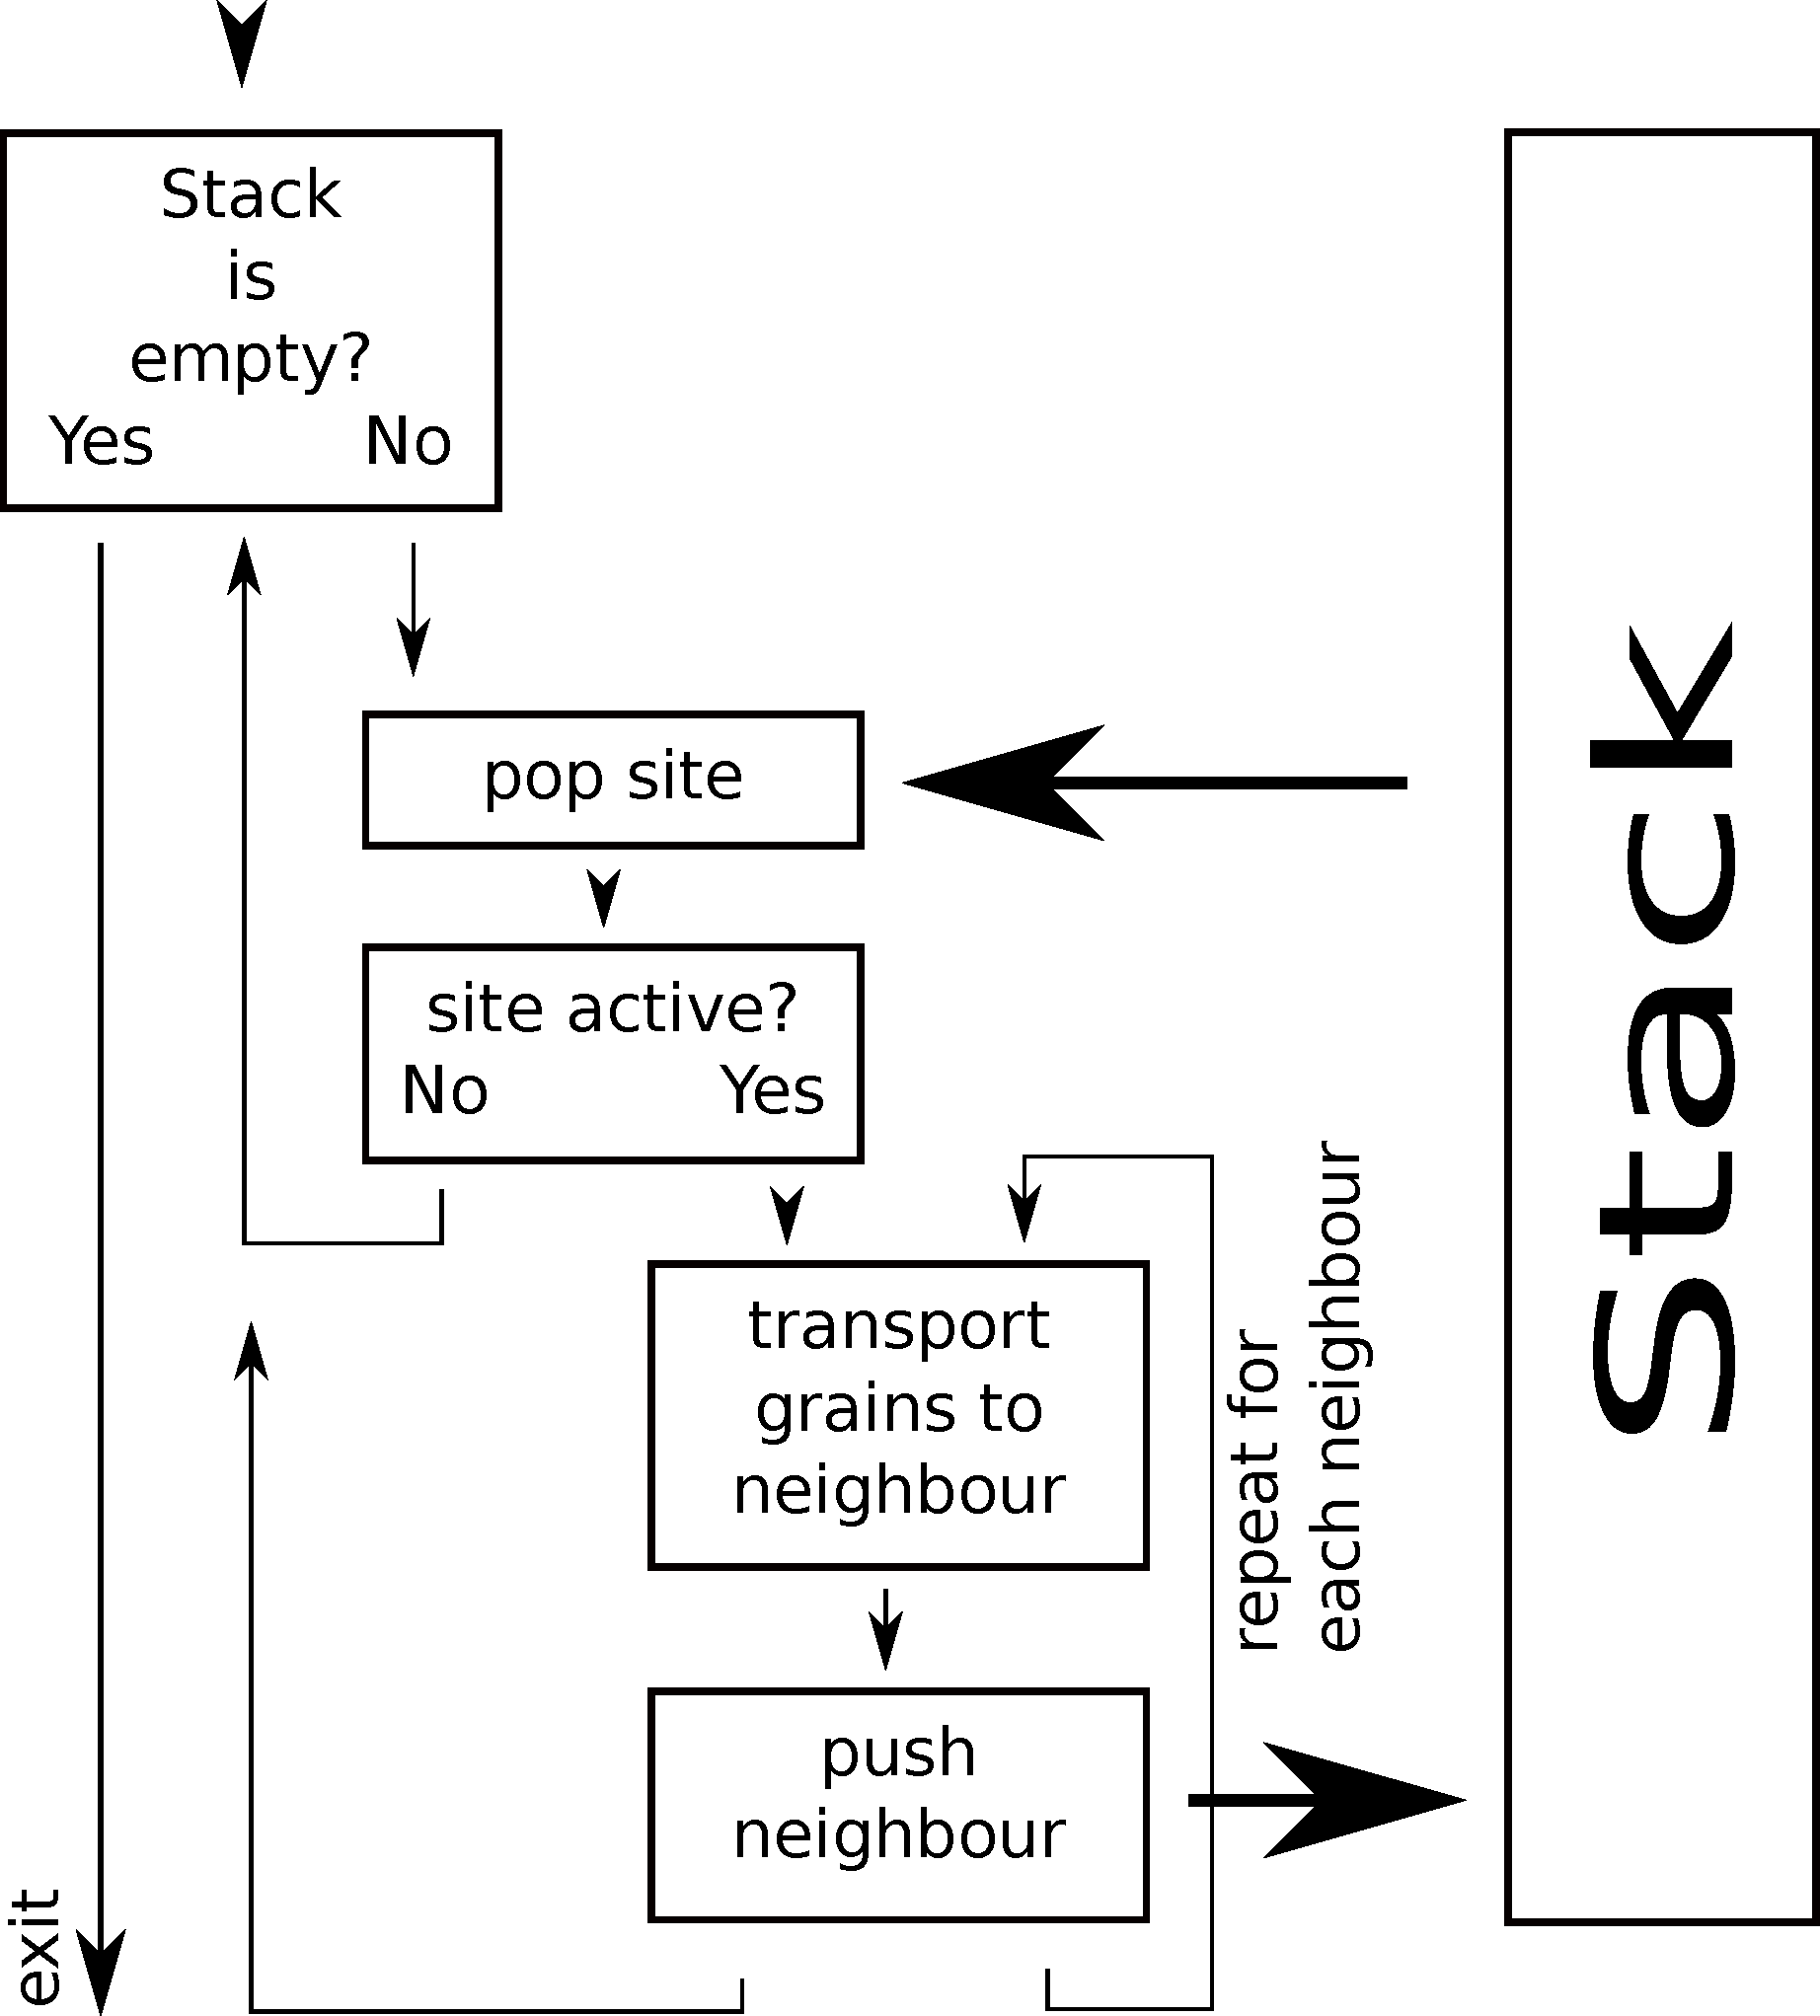
\includegraphics[width=0.5\textwidth]{pics/pic3_stack2.pdf}
\caption[]{using a stack for avalanche calculation}
\label{pics:stack2}
\end{figure}

Considering the example from figure \ref{pics:abelian}, the stack algorithm results in the following sequence:
\begin{enumerate}
 \setcounter{enumi}{-1}
 \item push C3
 \item pop C3, topple, push its neighbours (C2,C4,B3 and D3) to stack
 \item pop B3, topple, push B2, B4, A3 and C3 to stack
 \item pop B2, \ldots
 \item pop C2, \ldots
 \item pop B4, \ldots
 \item pop C4, \ldots
\end{enumerate}
Figure \ref{pics:stack1} shows the states of the stack after each of these steps. To avoid confusion, only the active sites are shown here.

\begin{figure}[!htpb]
\centering
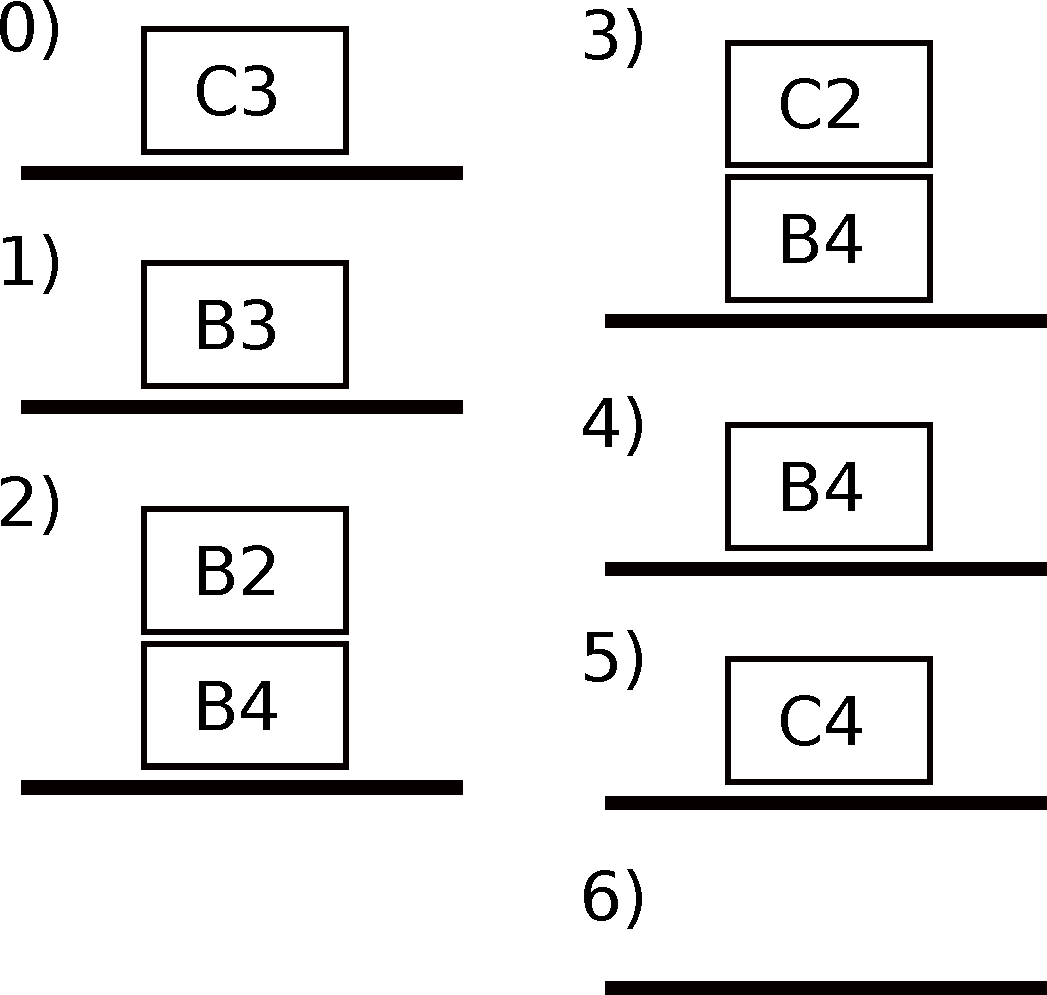
\includegraphics[width=0.5\textwidth]{pics/pic2_stack1.pdf}
\caption[]{A sample sequence of stack states. The algorithm proceeds until the stack is empty.}
\label{pics:stack1}
\end{figure}

The main loop including the stack feature looks like this:
\begin{lstlisting}
for t=1:timesteps
	% choose random site
	% ...

	% place grain
	% ...

	% push site to stack
	stack_n = 1;
	stack_x(1) = x;
	stack_y(1) = y;

	% avalanche - work through stack
	while (stack_n > 0)

		% pop from stack
		x = stack_x(stack_n);
		y = stack_y(stack_n);
		stack_n = stack_n - 1;

		% check if overcritical/active
		if (f(y,x) > critical_state)
			% collapse/topple
			f(y,x) = f(y,x) - neighbours * collapse;

			% look at every neighbour
			for n=1:neighbours
				% add/transport grain to neighbour
				f(y+neighbour_offset_y(n),x+neighbour_offset_x(n)) = ...
					f(y+neighbour_offset_y(n),x+neighbour_offset_x(n)) + collapse;

				% push neighbour to stack
				stack_n = stack_n + 1;
				stack_x(stack_n) = x + neighbour_offset_x(n);
				stack_y(stack_n) = y + neighbour_offset_y(n);
			end
		end
	end
end
\end{lstlisting}


\section{Statistics}\label{chp3:statistics}
Many different variables may be of interest for the statistical analysis of sandpile models. The easiest to implement is avalanche size:

\begin{lstlisting}
...

% check if overcritical/active
if (f(y,x) > critical_state)

	% collapse/topple
	f(y,x) = f(y,x) - neighbours * collapse;

	% record statistics
	avalanche_sizes(t) = avalanche_sizes(t) + 1;

	...
\end{lstlisting}

Here, the number of avalanches is recorded at every time step by increasing the counter after each toppling that happens during the avalanche. After the main loop, the data is sorted and the distribution is fitted into a power-law distribution given by
\[
P(s) = a \cdot s^b
\]
where $P$ is the number of avalanches of size $s$. The coefficients $a$ and $b$ are determined using a simple solver that minimizes $a \cdot s^b-P(s)$.

\begin{lstlisting}
% count avalanche sizes - calculate distribution
for s=1:max(avalanche_sizes)
	avalanche_count(s) = size(avalanche_sizes(avalanche_sizes==s),2);
end

% filter zero values
s = [1:max(avalanche_sizes)];
P = avalanche_count(1:end);
s = s(P>0);
P = P(P>0);

% fit into power-law
[c,fval,info,output]=fsolve(@(c)((c(1).*s.^c(2))-P),[100,1]);
a = c(1);
b = c(2);

\end{lstlisting}

In order to implement statistics of avalanche lifetime in the stack code, the number of additional (i.e. more than one) topplings per timestep must be counted. The reason for this is that the stack algorhithm does not follow a timescale and therefore the number of timesteps taken by an avalanche cannot be counted directly. Therefore, the following equation is used:
\[
s = \sum _t n = \underbrace{\sum_t (n - 1)}_{a} + \sum _t
\qquad \Rightarrow \sum _t = s - a
\]
where $s$ is the avalanche size, $t$ is the avalanche lifetime, $n$ is the number of topplings per timestep and $a$ is the total number of additional topplings. The neighbour-checking part of the stack loop looks like this:
\begin{lstlisting}
% count future topplings to be caused by this toppling
future_topplings = 0;

% look at every neighbour
for n=1:neighbours

	% add/transport grain to neighbour
	% ...

	% push neighbour to stack
	% ...

	% count future topplings to be caused by this toppling
	if (f(y+neighbour_offset_y(n),x+neighbour_offset_x(n)) == (critical_state+1))
		% i.e. if neighbour site becomes active
		future_topplings = future_topplings + 1;
	end

end
% calculate additional topplings caused
if (future_topplings > 0)
	avalanche_add(t) = avalanche_add(t) + future_topplings - 1;
end
\end{lstlisting}
For each toppling, the number of further topplings is counted, summed up and subtracted by one. Then, the avalanche lifetime is calculated according to the formula $\sum _t = s - a$ as follows:
\begin{lstlisting}
% return avalanche lifetimes
at = avalanche_sizes - avalanche_add;
\end{lstlisting}

\section{Implementation for $d$-dimension}

The generalization to $d$-dimension is quite straightforward using the linearized index, i.e., ennumerate the sites with one integer number. 
This is done using the relation:
\[
 v=(x_d-1)n^d+(x_{d-1}-1)n^{d-1}+\cdots+(x2-1)n+x1
\]
which is implemented in the function \texttt{linear_index(x,d,n)}, where \texttt{x} is the array with the coordinate of the lattice site. 



The inverse function is \texttt{coordinate(v,d,n)}, and is written using the Matlab modulus function \texttt{mod()}.
The idea is simple as well, as we can find a recurrent relation:
\[
v=v_d=(x_d-1)n^d+v_{d-1}=(x_d-1)n^d+(x_{d-1}-1)n^{d-1}+v_{d-2}=\cdots=(x_d-1)n^d+(x_{d-1}-1)n^{d-1}+\cdots+(x2-1)n+v_1
\]
hence, 
\[
 (x_d-1)=mod(v_d-v_{d-1},n^d); \quad  x_1=v_1
\]

The code for this is:
\begin{lstlisting}
x=zeros(1,d);    % coordinates (x(1),x(2),..., x(d))
va=zeros(1,d+1); 
va(d+1)=v-1;
  for i=d:-1:1   
    va(i)=mod(va(i+1),power(n,i-1));
    x(i)=1+(va(i+1)-va(i))/power(n,i-1);
  end  
end
\end{lstlisting} 

The nearest neighbour function for $d$-dimensional case is implemented in \texttt{neighbour(v,d,n,periodic_boundary)} function,
which gives the coordinates of the $2d$ nearest neighbour of a given site $v$.  
We also added the option of periodic boundary (write \texttt{1} in the argument) or finite boundary (\texttt{0}). 
Basically, the code consists of, first, give the coordinate of any site $v$ using \texttt{coordinate(v,d,n)} function, 
then, it distinguishes \emph{forward} and \emph{backward} neighbours, by adding or substracting $1$ respectively. 
In the periodic boundary case, when the coordinate is $0$ or bigger than $n$ (in fact, equal to $n+1$), then, the coordinates are set to
$n$ or $1$, respectively.  For the finite boundary, we set all the coordinates outside the lattice equal to $-n^d$, 
since this will always give the corresponding $v<0$, therefore, in the main program, we can easily exclude them using an \texttt{if} condition true for $v>0$. 
The exact code for this function is attached in the Appendix.

\section{Real field sandpile}

So far we have discussed the sandpile model considering a discrete field, interpreted as height, and adding value $1$ to the field of a random site for each driving time. 
We can think of this case as a field of grains of uniform size, however, it is straightforward to generalize it to a real field, 
where we can interpret it as grains with different sizes (or preferably thinking in terms of energy).
It can be done by adding a \emph{real} random value between $0$ and $1$, to the field in each driving time. 


When the site is overcritical, its nearest neighbours receive a grain of a random size as well, then summing up these numbers, it is what the toppling site loses (conservative case).
This implies closed boundary for this case, hence it is preferable to introduce some friction if we wish to study the system for a large driving time, just to avoid very large avalanches,
as there will be a point where all the sites will be overcritical, like the periodic boundary case. 
The friction parameter \texttt{f} means that there is some energy lost in the propagation to the neighbouring sites.
i.e., for \texttt{f<1}, it corresponds to the dissipative case, 
with an energy lost of $\Delta E=(1-f)E$, where $E$ is the value of the field for the conservative case (\texttt{f=1}).

The basic code is rewritten here as:
\begin{lstlisting}
c=0;
for k=1:2*d
  r(k)=rand(1);                    
  E(vnn)=E(vnn)+r(k); 
  c=c+r(k);
end        
E(v)=(E(v)-c)*f;
\end{lstlisting}
where \texttt{c} is the sum of the energy values that each nearest neighbour site \texttt{vnn} gained when the site \texttt{v} relaxed. 



The whole sandpile program for $d$-dimension is a bit more sophisticated, using also the \emph{stack} method discussed before, 
but here, there is a stack for each parallel sites dropping caused by one initial toppling site. The advantage is that we can count also the lifetime of the avalanche. 
The whole program is attached in the Appendix, and more details are commented in there. The discrete field is also implemented there. 
Some more comments are written in the code itself.

This real field case makes our sandpile model a bit more realistic, though still, the we have finite digits, hence, it is equivalent to the discrete case, only with different propagation rules.
Besides, the lattice sites are also discrete.






